\chapter{Summary and Outlook}

\label{ch:conclusion}

The search described herein targetted the unique signature of \TeV-scale, charged \acp{LLP}, which are predicted in a variety of extensions to the \ac{SM} including some versions of \ac{SUSY}.
The dataset of 13 \TeV proton-proton collisions was collected during 2015 by the ATLAS detector at the \ac{LHC}, with an integrated luminosity of \lumi~fb\tsup{-1}.
The specific search strategy focused on identifying massive, charged particles which propagate through the Pixel detector in ATLAS by their characteristically large ionization.
Recent updates to the strategy also include a number of rejection techniques that significantly reduce \ac{SM} backgrounds compared to previous iterations.
The analysis also provided a data-driven background estimation method that was shown to be effective with validation tests in both simulation and actual data.

No significant excesses above the background prediction were found in the data, and so limits were placed on the production of massive, charged, \acp{LLP}.
Using a benchmark model of simulated \rhadrons, cross sections above 10-100 fb were excluded at 95\% confidence level, depending on the lifetime of the \rhadron.
Together with the predicted gluino pair-production cross sections, these lead to mass limits on \rhadrons up to 1600 \GeV where the search is most sensitive.
Though these specific values assume an \rhadron \ac{LLP}, the search strategy accomodates a number of other species and the limits can be interpreted for other models.

This search plays an important role in the current, combined ATLAS search for long lived particles.
The mass limits provided by various ATLAS searches for long-lived gluino \rhadrons can be seen in Figure~\ref{fig:combined_rhadrons}.
This search provides the most competitive limit for lifetimes between 3 ns up through very long lifetimes, where it is still competitive with dedicated searches for \ac{VLL} particles.
The limits placed on gluino production are very similar to the limits on promptly decaying models.

\begin{figure}[htbp]
\centering
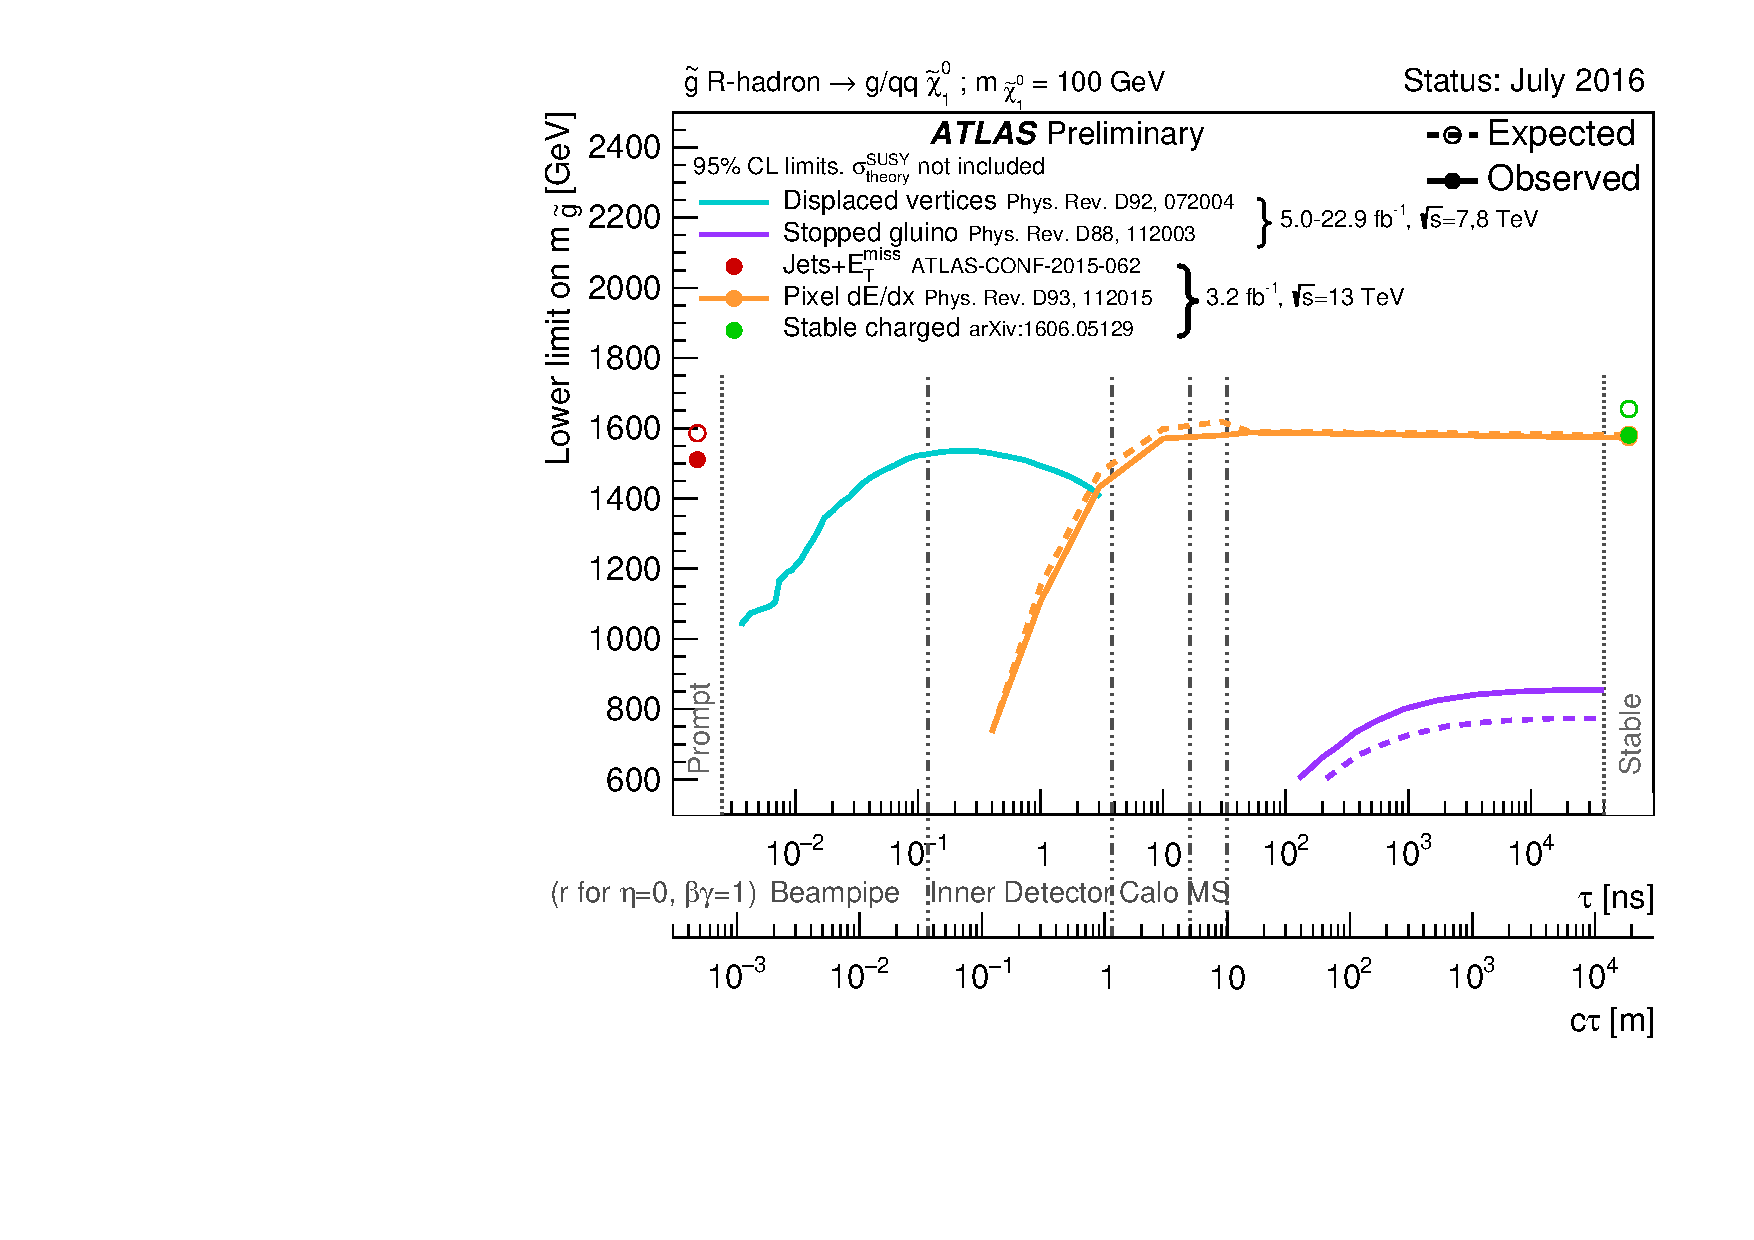
\includegraphics[width=\fullfig]{figures/combined_rhadrons.pdf}  
\caption{The constraints on the gluino mass as a function of lifetime for a split-supersymmetry model with the gluino \rhadrons decaying into a gluon or light quarks and a neutralino with mass of 100 GeV. The solid lines indicate the observed limits, while the dashed lines indicate the expected limits. The area below the curves is excluded. The dots represent results for which the particle is assumed to be prompt or \acs*{VLL}. This curve representing this analysis is shown in orange.}
\label{fig:combined_rhadrons}
\end{figure}

These results are expected to be significantly improved in the following years, primarily because of continuing data collection at 13 \TeV at the \ac{LHC}.
During 2016, but after the release of this analysis, ATLAS recorded an additional 35.5 fb\tsup{-1} of collisions, and analysis of this data would significantly extend the limits presented here.
The next iteration of the analysis can also provide additional interpretations of the search, by explicitly including other models like stop \rhadrons and charginos in the limit calculations, as has been done in previous searches~\cite{SUSY-2014-09}.
This strategy will continue to provide a competitive approach to discovering new \acp{LLP} throughout the lifetime of the \ac{LHC}.
